%-------------------------------------------------
% FileName: chapt-4.tex
% Author: Safin (zhaoqid@zsc.edu.cn)
% Version: 0.1
% Date: 2020-05-12
% Description: 第4章
% Others: 
% History: origin
%------------------------------------------------- 


% 断页
% \clearpage
\chapter{处理器相关技术设计}
第3章实现了RISC-V单周期处理器的设计,其中每条指令均在一个时钟周期内完成。然而,实际上,存储器的存取操作无法在一个周期内完成,即使采用最先进的SRAM工艺,也至少需要一个周期的存取延迟\cite{noguchi2008best}。因此,单周期处理器在实际中无法直接流片生产。

本章将在单周期处理器的基础上进行扩展,通过引入AXI4总线协议将其改造为多周期处理器。在此基础上,将在存储优化部分引入高速缓存技术,以提升访存效率;在并行优化部分引入流水线技术,以增强处理器的并行处理能力。

\section{总线}
计算机中的各个模块并非孤立运作,不同模块间的数据交换是系统正常运行的关键。例如,指令取指单元(IFU)与指令译码单元(IDU)之间、中央处理器(CPU)与内存控制器之间,均需遵循特定的通信协议以实现高效的数据传输。从广义上讲,总线可被视为一种通信系统,其核心功能在于协调不同模块间的数据流动。本节将专注于狭义上的总线设计,即模块间通信协议的制定。这一协议不仅定义了数据传输的格式和时序,确保数据的完整性和可靠性。通过精心设计的通信协议,可以显著提升系统的整体性能和可扩展性。

\subsection{内部总线}
在处理器内部,各单元间需相互通信。通常,主动发起通信的模块称为主设备(master),而响应通信的模块称为从设备(slave)。然而,主设备无法保证每个周期都能向从设备发送消息(例如,IFU无法在每个周期内取到指令),从设备也无法确保每个周期都能处理主设备的消息(例如,EXU无法在一个周期内完成运算)。这种不确定性体现了异步通信的特性,即两个模块之间的通信时机无法预先确定。

\begin{figure}[htbp]
	\centering
	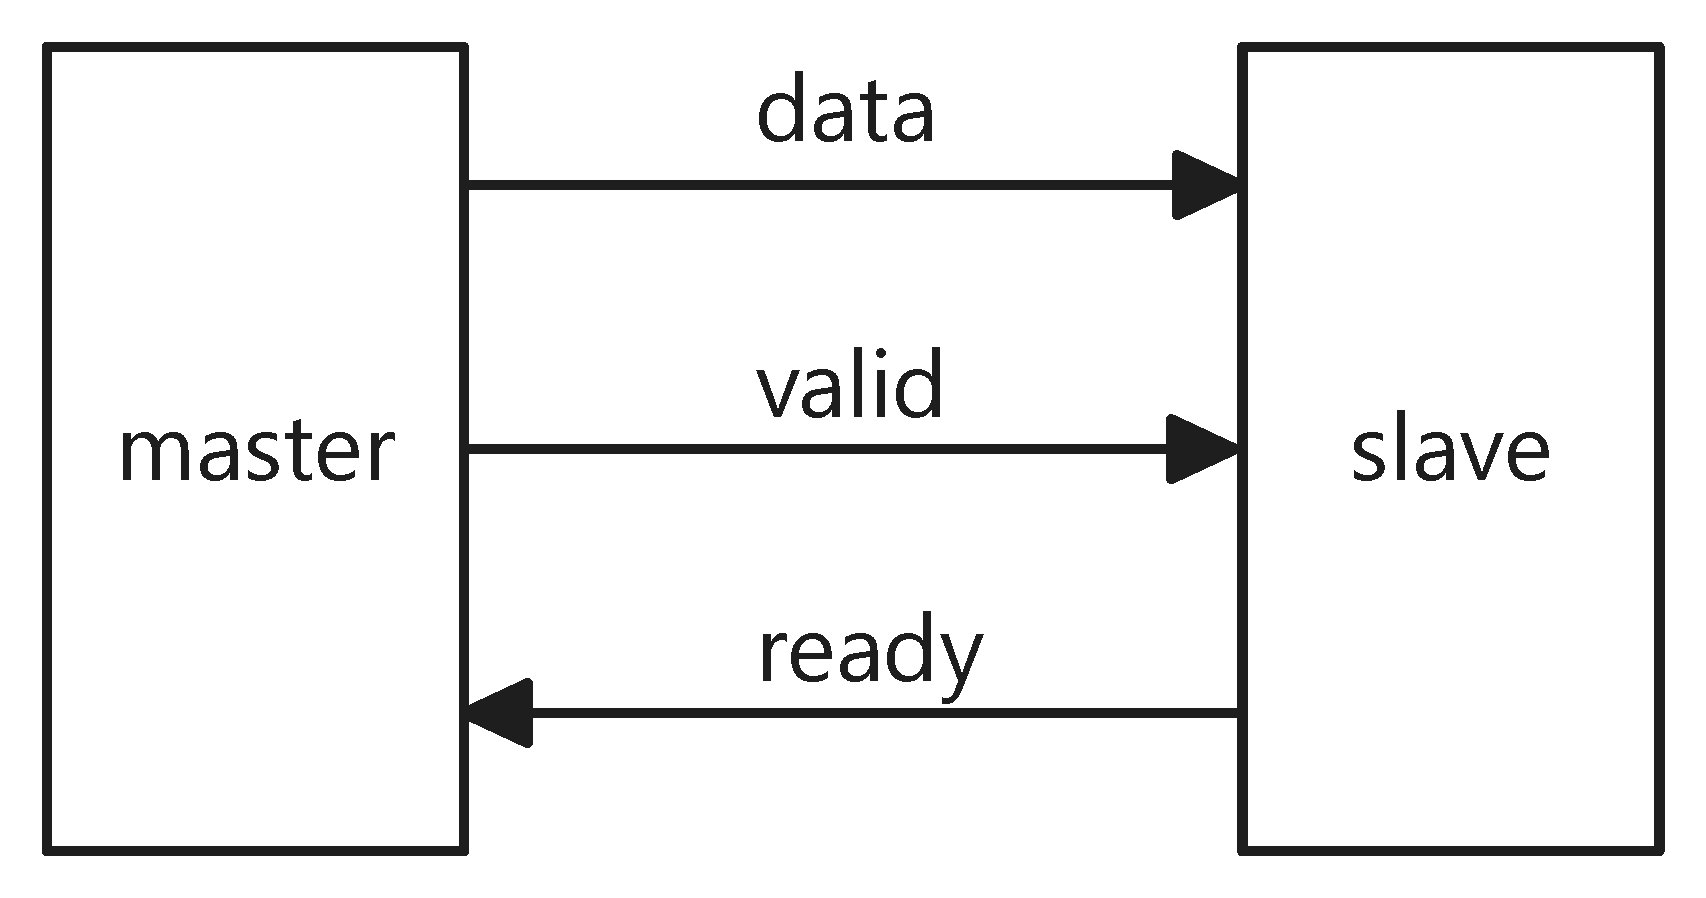
\includegraphics[width=0.5\textwidth]{image/handshake.pdf}
	\caption{模块间通信的握手协议}
	\label{fig:handshake}
\end{figure}

为确保异步通信中数据传输的准确性,需设计一种握手协议。如图\ref{fig:handshake}所示,该协议包含三种信号:data是主设备向从设备发送的数据;valid:表示发送的数据有效;ready表示从设备准备好接收数据。通信仅在valid和ready信号同时有效时发生。这种机制不仅实现了异步通信,还增强了通信协议的灵活性,确保了数据传输的可靠性和高效性。

关于通信逻辑的设计,握手双方需依据握手信号的不同情况进入相应状态并采取操作。为此,需设计一个有限状态自动机,其状态转移如图\ref{fig:handshake_automata}所示:

\begin{enumerate}[label={\arabic*)}, itemsep=0pt, parsep=0pt]
	\item master初始处于空闲状态idle,此时将valid信号置为无效。
	      \begin{itemize}
		      \item 如果无需发送消息,则持续保持idle状态。
		      \item 若需发送消息,则将valid信号置为有效,并转入wait\_ready状态。
	      \end{itemize}
	\item master处于wait\_ready状态时,需检测来自slave的ready信号。
	      \begin{itemize}
		      \item 若ready信号无效,则继续停留在wait\_ready状态。
		      \item 一旦ready信号有效,表明握手成功,随即向slave发送消息,并返回idle状态。
	      \end{itemize}
\end{enumerate}

\begin{figure}[htbp]
	\centering
	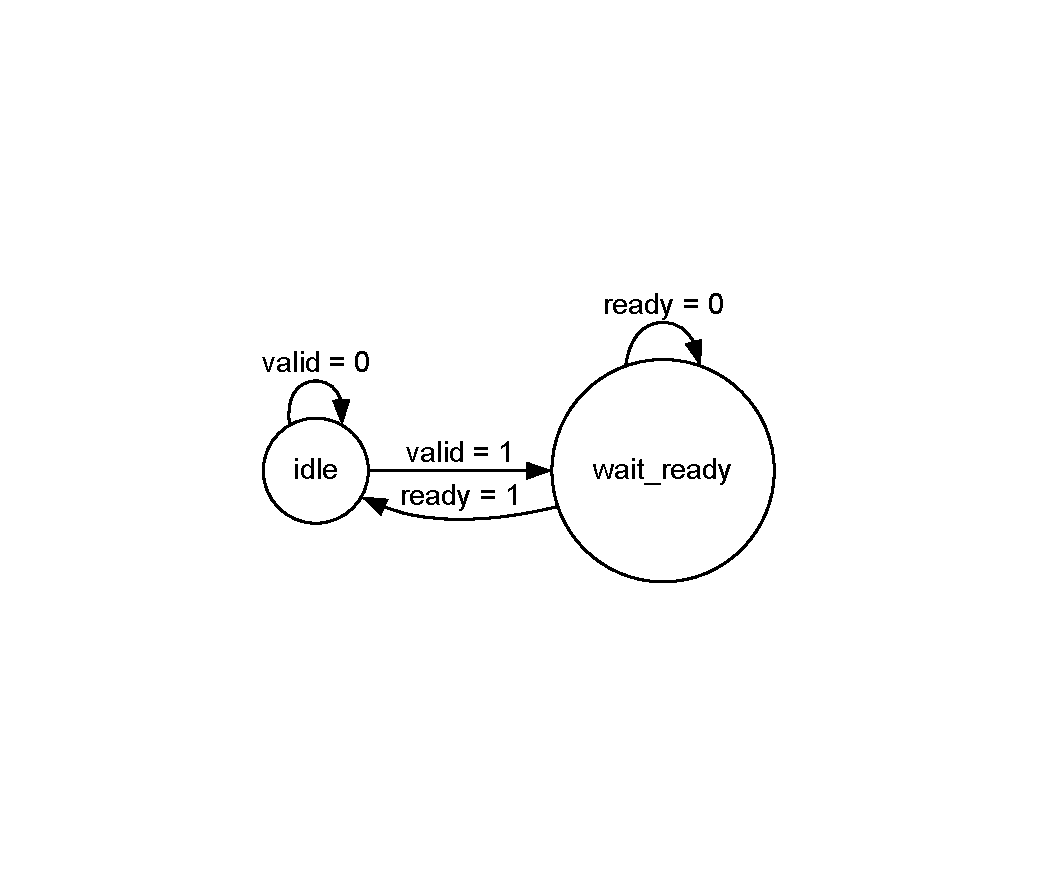
\includegraphics[width=0.6\textwidth]{image/handshake_automata.pdf}
	\caption{master的有限状态自动机设计}
	\label{fig:handshake_automata}
\end{figure}

在单周期处理器的基础上,如图\ref{fig:multicycle_cpu}所示,通过在有数据交换的单元模块之间引入握手信号,可以有效管理模块间的通信。对于单周期处理器,每个周期内上游模块发送的消息都被视为有效,而下游模块始终处于就绪状态以接收新消息。这种设计假设所有模块都能在一个周期内完成其任务,这在实际应用中可能并不现实。

相比之下,多周期处理器采用更为灵活的通信机制。在多周期处理器中,当上游模块空闲时,它不会发送有效消息,而下游模块在忙碌时也不会接收新消息。这种机制允许模块根据自身处理速度进行通信,避免了不必要的等待和资源浪费。特别地,IFU会在收到WBU的完成信号后,才取下一条指令,确保了数据传输的准确性和处理器操作的有序性。这种基于握手信号的通信协议,不仅提高了处理器的灵活性和效率,还为处理复杂操作提供了必要的支持。

\begin{figure}[htbp]
	\centering
	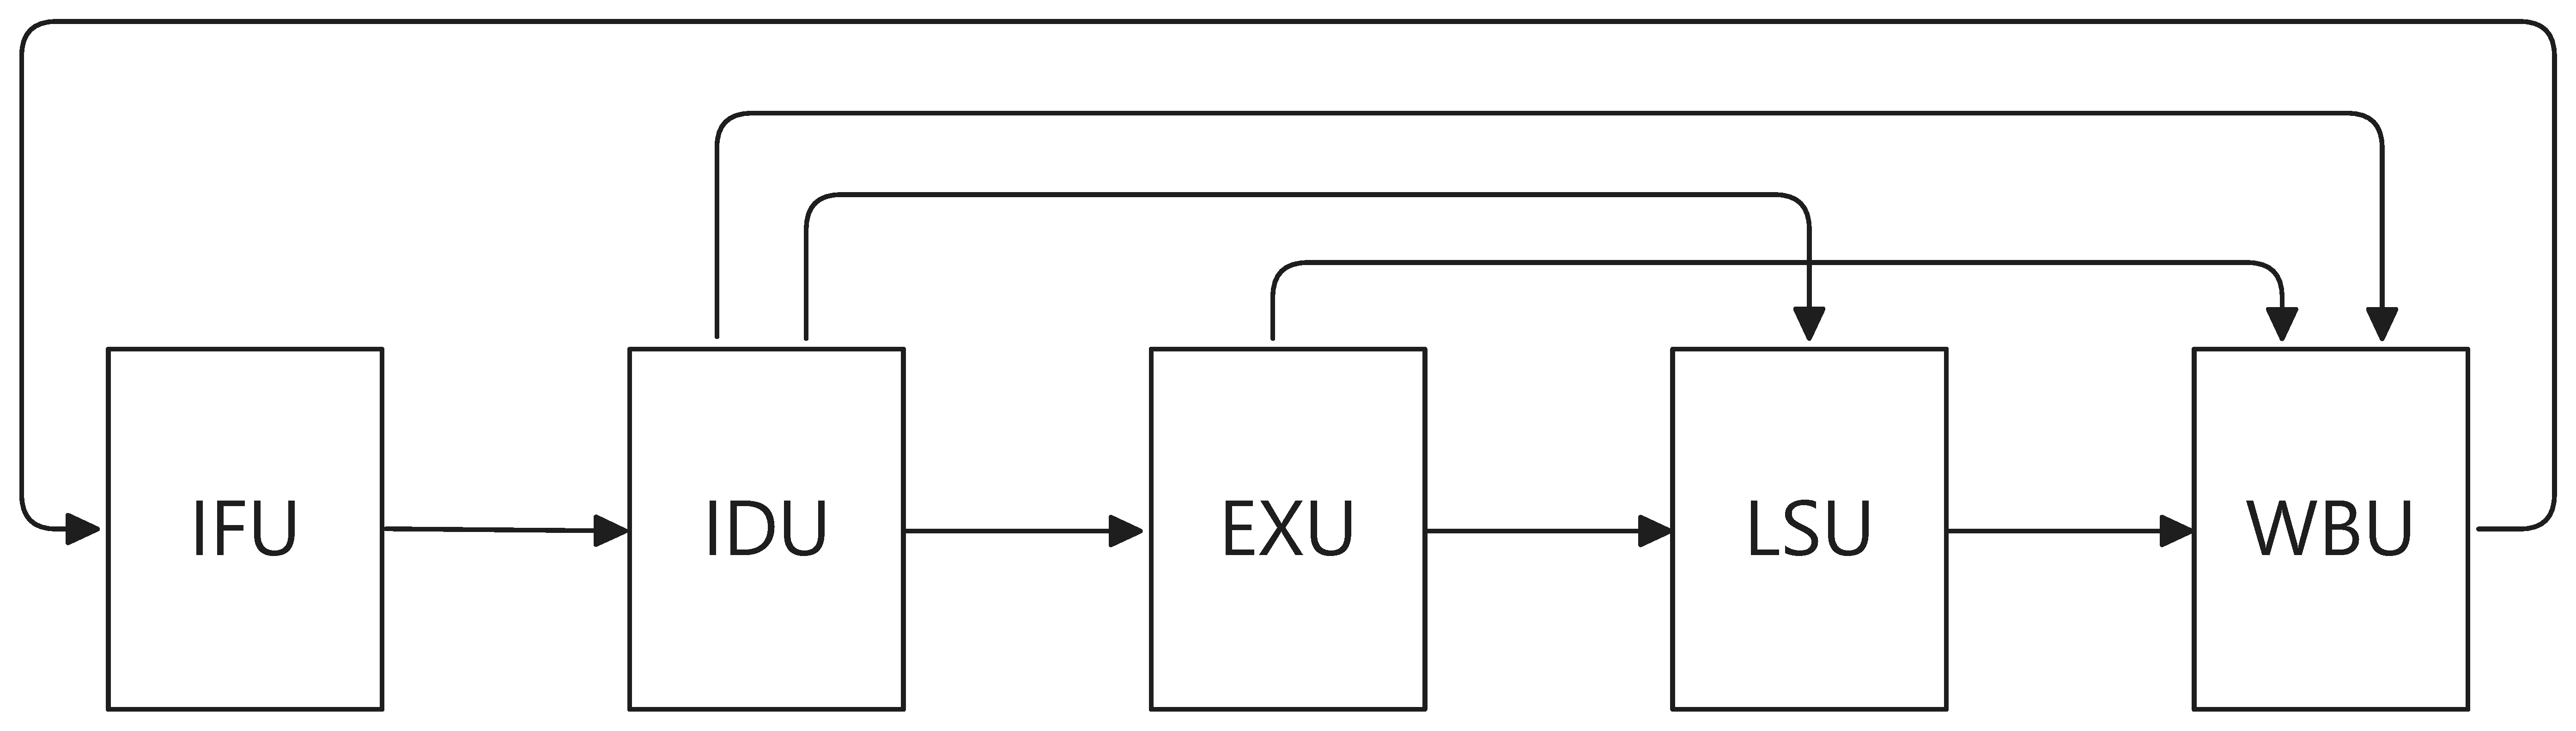
\includegraphics[width=0.8\textwidth]{image/multicycle_cpu.pdf}
	\caption{多周期处理器结构图}
	\label{fig:multicycle_cpu}
\end{figure}

如图\ref{fig:centralized_controller}所示,集中式控制处理器通常显得较为累赘,尤其是在模块数量和复杂度不断增加的情况下。这种控制方式需要一个全局控制器来收集所有模块的状态信息,并据此来协调各个模块的下一步操作。可以将集中控制器视为一个大型的有限状态自动机,它通过一个全局的状态机来管理各个模块的状态,从而控制模块间的通信并决定下一个状态。然而,这种集中式的方法在可扩展性方面存在明显不足,因为随着系统规模的扩大,控制器的设计复杂度会呈指数级增长,需要考虑每个模块不同状态的组合,这使得统一决策变得异常困难。

\begin{figure}[htbp]
	\centering
	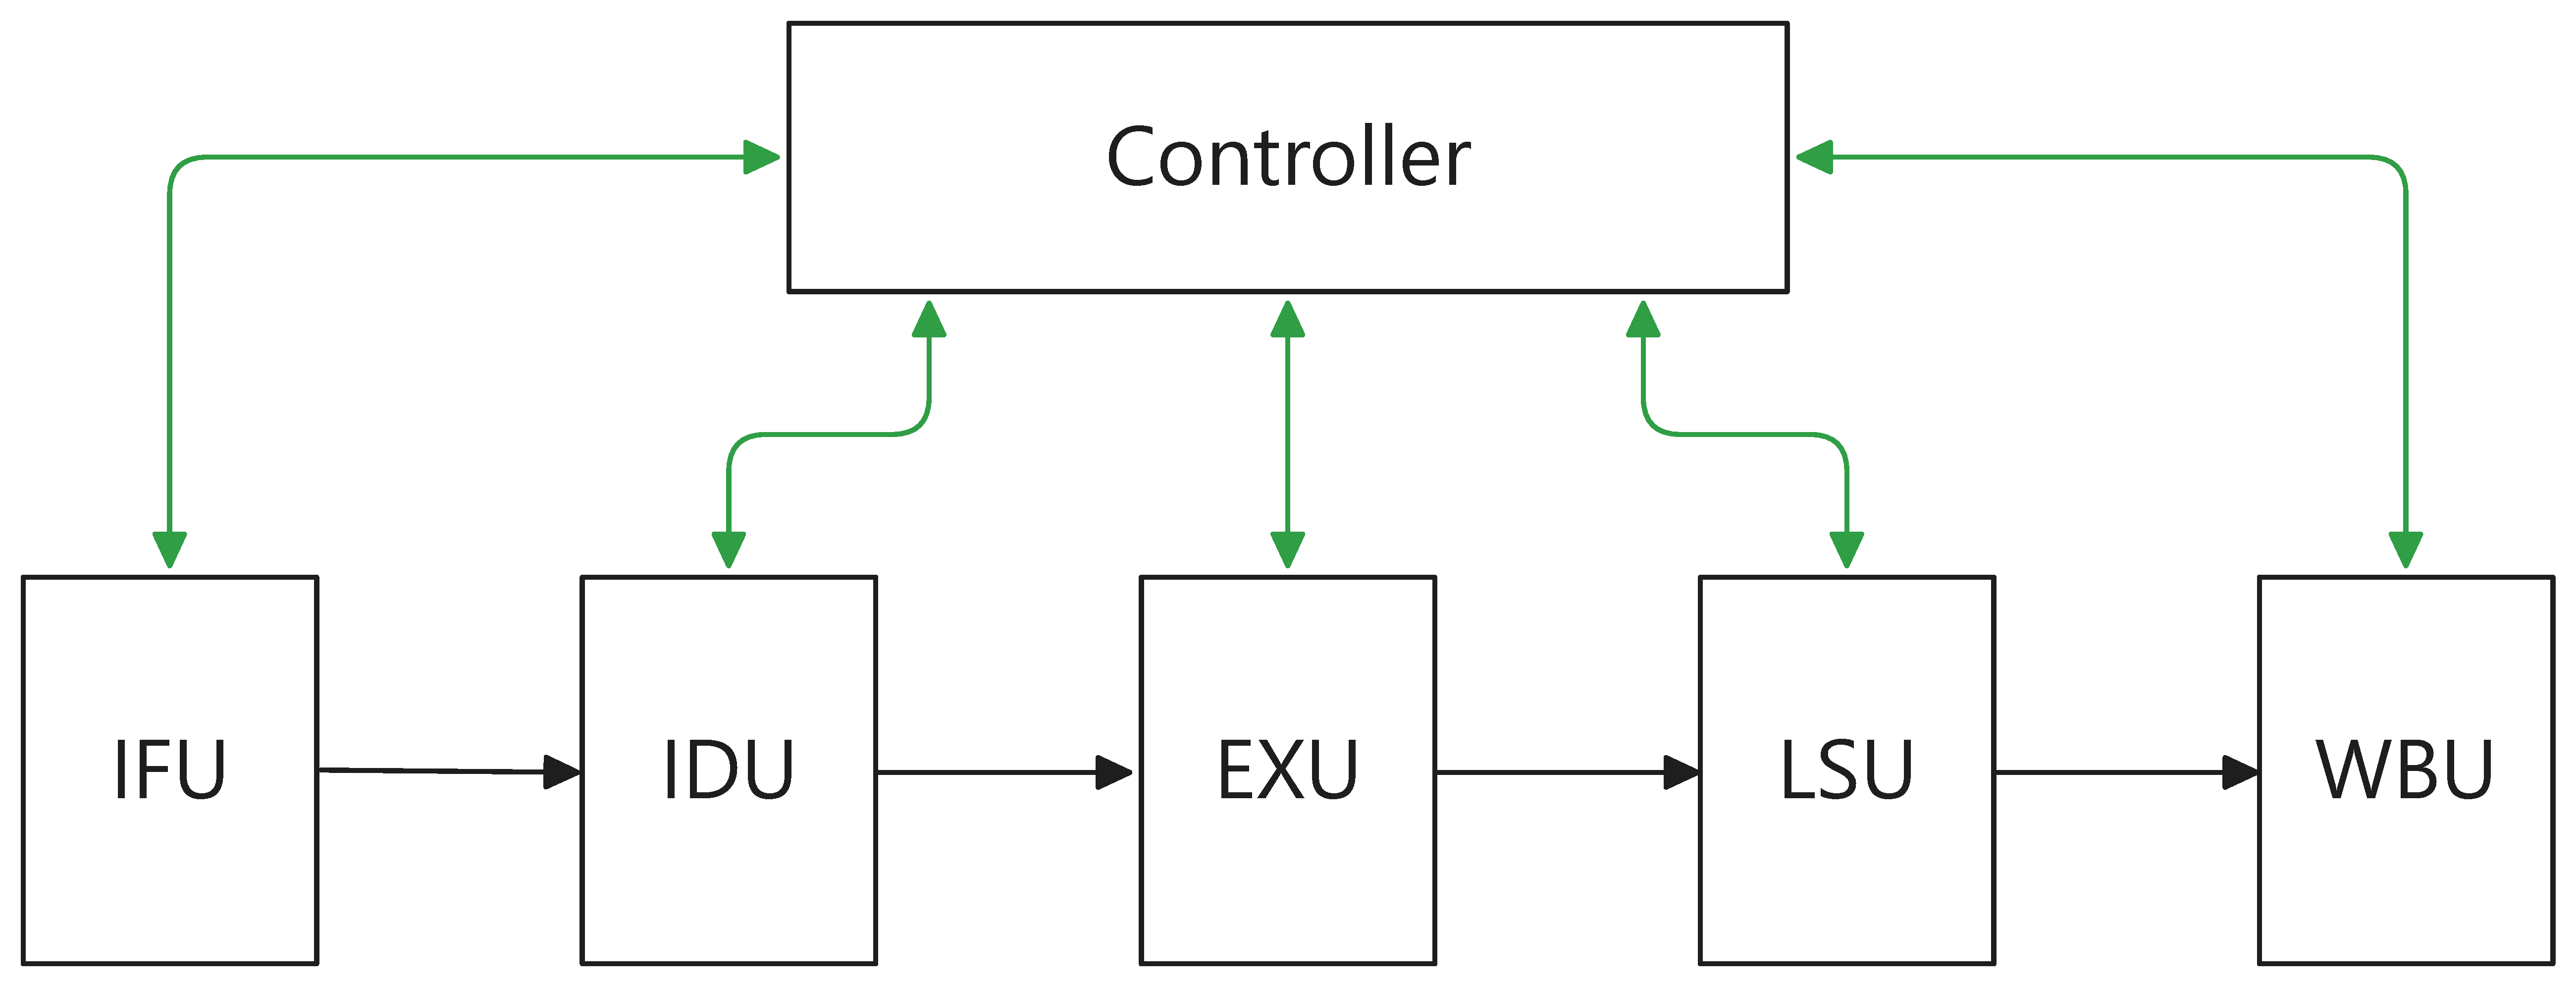
\includegraphics[width=0.8\textwidth]{image/centralized_controller.pdf}
	\caption{集中控制处理器结构图}
	\label{fig:centralized_controller}
\end{figure}

所以,基于握手的分布式控制提供了一种更为灵活和可扩展的解决方案。在这种方法中,每个模块的行为仅取决于自身的状态以及下游模块的状态。这种局部通信机制允许各个模块相对独立地运作,从而简化了整体设计。分布式控制不仅提高了系统的可扩展性,还使得处理器结构的修改和扩展变得更加容易,因为每个模块可以独立地进行调整和优化,而不会对整个系统造成过多的影响。这种模块化的设计理念,使得处理器能够更好地适应不断变化的需求和日益增长的复杂性。

\subsection{系统总线}
处理器不仅需要建立内部模块间的通信,还需要与外围设备(如存储器、时钟和串口等)进行通信。为了实现这一目标,系统总线扮演着至关重要的角色。本小节将介绍AXI4(Advanced eXtensible Interface 4)总线协议,该协议是ARM的AMBA(Advanced Microcontroller Bus Architecture)规范的一部分\cite{amba2011axi},旨在提供一种灵活、高效的方式来连接处理器、存储器和外设。

AXI4总线协议以其高效性和灵活性著称,特别适用于复杂系统设计。它通过五条独立的传输通道(读地址通道、写地址通道、读数据通道、写数据通道和写响应通道)实现高效的通信机制,这些通道仅支持单向传输,确保了数据传输的高效性和可靠性。通过这种架构,AXI4总线能够有效地管理数据流,减少通信延迟,并提高系统的整体性能。其灵活的配置选项使其适用于各种规模和复杂度的系统设计,从而成为现代处理器设计中的首选总线协议之一。简单来说,AXI4总线是为每种传输数据加上了valid和ready握手信号。

读地址通道用于从主设备到从设备的读请求地址传输,其信号描述如表\ref{tab:read_address_bus}所示。

\begin{table}[H]
	\centering
	\caption{读地址通道信号描述表}
	\begin{tabularx}{\textwidth}{>{\centering\arraybackslash}p{4cm} >{\centering\arraybackslash}p{3cm} >{\centering\arraybackslash}X}
		\toprule
		\textbf{信号名} & \textbf{源} & \textbf{描述}        \\
		\midrule
		ARVALID      & 主设备        & 表示主设备已准备好发送读地址信息   \\
		ARREADY      & 从设备        & 表示从设备已准备好接收读地址信息   \\
		ARADDR       & 主设备        & 读操作的目标地址           \\
		ARLEN        & 主设备        & 传输的长度,表示一次读操作的传输次数 \\
		ARSIZE       & 主设备        & 传输的大小,表示每次传输的数据宽度  \\
		ARBURST      & 主设备        & 突发类型,描述传输的模式。      \\
		ARID         & 主设备        & 事务标识符,用于标识不同的读操作   \\
		\bottomrule
	\end{tabularx}
	\label{tab:read_address_bus}
\end{table}

写地址通道用于从主设备到从设备的写请求地址传输,其信号描述如表\ref{tab:write_address_bus}所示。

\begin{table}[H]
	\centering
	\caption{写地址通道信号描述表}
	\begin{tabularx}{\textwidth}{>{\centering\arraybackslash}p{4cm} >{\centering\arraybackslash}p{3cm} >{\centering\arraybackslash}X}
		\toprule
		\textbf{信号名} & \textbf{源} & \textbf{描述}        \\
		\midrule
		AWVALID      & 主设备        & 表示主设备已准备好发送写地址信息   \\
		AWREADY      & 从设备        & 表示从设备已准备好接收写地址信息   \\
		AWADDR       & 主设备        & 写操作的目标地址           \\
		AWLEN        & 主设备        & 传输的长度,表示一次写操作的传输次数 \\
		AWSIZE       & 主设备        & 传输的大小,表示每次传输的数据宽度  \\
		AWBURST      & 主设备        & 突发类型,描述传输的模式。      \\
		AWID         & 主设备        & 事务标识符,用于标识不同的写操作   \\
		\bottomrule
	\end{tabularx}
	\label{tab:write_address_bus}
\end{table}

读数据通道用于从设备到主设备的读数据响应,其信号描述如表\ref{tab:read_data_bus}所示。

\begin{table}[H]
	\centering
	\caption{读数据通道信号描述表}
	\begin{tabularx}{\textwidth}{>{\centering\arraybackslash}p{4cm} >{\centering\arraybackslash}p{3cm} >{\centering\arraybackslash}X}
		\toprule
		\textbf{信号名} & \textbf{源} & \textbf{描述}       \\
		\midrule
		RVALID       & 从设备        & 表示从设备已准备好发送读数据信息  \\
		RREADY       & 主设备        & 表示主设备已准备好接收读数据信息  \\
		RDATA        & 从设备        & 读操作返回的数据          \\
		RRESP        & 从设备        & 响应类型,用于描述读操作的状态   \\
		RLAST        & 从设备        & 表示当前数据是读操作的最后一个数据 \\
		RID          & 从设备        & 事务标识符,用于标识不同的读操作  \\
		\bottomrule
	\end{tabularx}
	\label{tab:read_data_bus}
\end{table}

写数据通道用于从主设备到从设备的写数据传输,其信号描述如表\ref{tab:write_data_bus}所示。

\begin{table}[H]
	\centering
	\caption{写数据通道信号描述表}
	\begin{tabularx}{\textwidth}{>{\centering\arraybackslash}p{4cm} >{\centering\arraybackslash}p{3cm} >{\centering\arraybackslash}X}
		\toprule
		\textbf{信号名} & \textbf{源} & \textbf{描述}       \\
		\midrule
		WVALID       & 主设备        & 表示主设备已准备好发送写数据信息  \\
		WREADY       & 从设备        & 表示从设备已准备好接收写数据信息  \\
		WDATA        & 主设备        & 写操作的数据            \\
		WSTRB        & 主设备        & 写选通,用于指示数据的哪些字节有效 \\
		WLAST        & 主设备        & 表示当前数据是写操作的最后一个数据 \\
		WID          & 主设备        & 事务标识符,用于标识不同的写操作  \\
		\bottomrule
	\end{tabularx}
	\label{tab:write_data_bus}
\end{table}

写响应通道用于从设备到主设备的写操作状态响应,其信号描述如表\ref{tab:write_response_bus}所示。

\begin{table}[H]
	\centering
	\caption{写响应通道信号描述表}
	\begin{tabularx}{\textwidth}{>{\centering\arraybackslash}p{4cm} >{\centering\arraybackslash}p{3cm} >{\centering\arraybackslash}X}
		\toprule
		\textbf{信号名} & \textbf{源} & \textbf{描述}         \\
		\midrule
		BVALID       & 从设备        & 表示从设备已准备好发送写响应信息    \\
		BREADY       & 主设备        & 表示主设备已准备好接收写响应信息    \\
		BRESP        & 从设备        & 写操作的响应类型,用于描述写操作的状态 \\
		BID          & 从设备        & 事务标识符,用于标识不同的写操作    \\
		\bottomrule
	\end{tabularx}
	\label{tab:write_response_bus}
\end{table}

关于AXI4总线的握手机制只有一种(valid和ready信号),若在时钟上升沿检测到valid和ready信号同时有效,此时消息有效,下一周期valid和ready信号将置为无效。如图\ref{fig:handshake_wave}所示,根据valid和ready信号的先后顺序,将会出现三种时序关系。

\begin{figure}[htbp]
	\centering
	\subfigure[ready和valid同时到达]{
		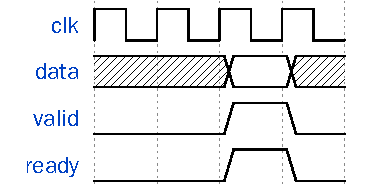
\includegraphics[width=0.31\textwidth]{image/handshake_wave_a.pdf}
		\label{fig:handshake_wave_a}
	}
	\subfigure[valid比ready先到达]{
		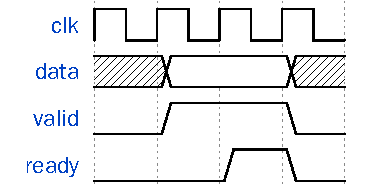
\includegraphics[width=0.31\textwidth]{image/handshake_wave_b.pdf}
		\label{fig:handshake_wave_b}
	}
	\subfigure[ready比valid先到达]{
		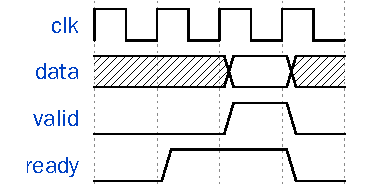
\includegraphics[width=0.31\textwidth]{image/handshake_wave_c.pdf}
		\label{fig:handshake_wave_c}
	}
	\caption{不同情况下的握手时序图}
	\label{fig:handshake_wave}
\end{figure}

\begin{enumerate}[label={\arabic*)}, itemsep=0pt, parsep=0pt]
	\item \textbf{双方同时准备就绪}:若发送方和接收方同时将valid和ready信号置为有效,数据传输立即开始,完成该次传输任务。
	\item \textbf{发送方先准备就绪}:若发送方先将valid信号置为有效,表示数据或地址及控制信号已准备就绪,发送方需维持这些信号直至接收方将ready信号置为有效,从而完成数据传输。
	\item \textbf{接收方先准备就绪}:若接收方先将ready信号置为有效,表示已准备好接收数据,发送方随后需将数据或地址及控制信号准备就绪,并将valid信号置为有效,以完成传输。
\end{enumerate}

至此,单周期处理器已成功优化为多周期处理器。内部总线负责协调处理器内部各模块间的通信,而系统总线则负责处理器与外部设备之间的通信。如图\ref{fig:bus}所示,该多周期处理器的总线结构通过仲裁器(Arbiter)将指令取指单元(IFU)和访存单元(LSU)连接到CPU外部的AXI4总线接口。该接口随后连接到信号路由器(XBar),通过XBar将信号精确路由至相应的外部设备,从而实现高效的数据传输和设备通信。这种设计确保了处理器内部和外部通信的高效性和灵活性。

\begin{figure}[htbp]
	\centering
	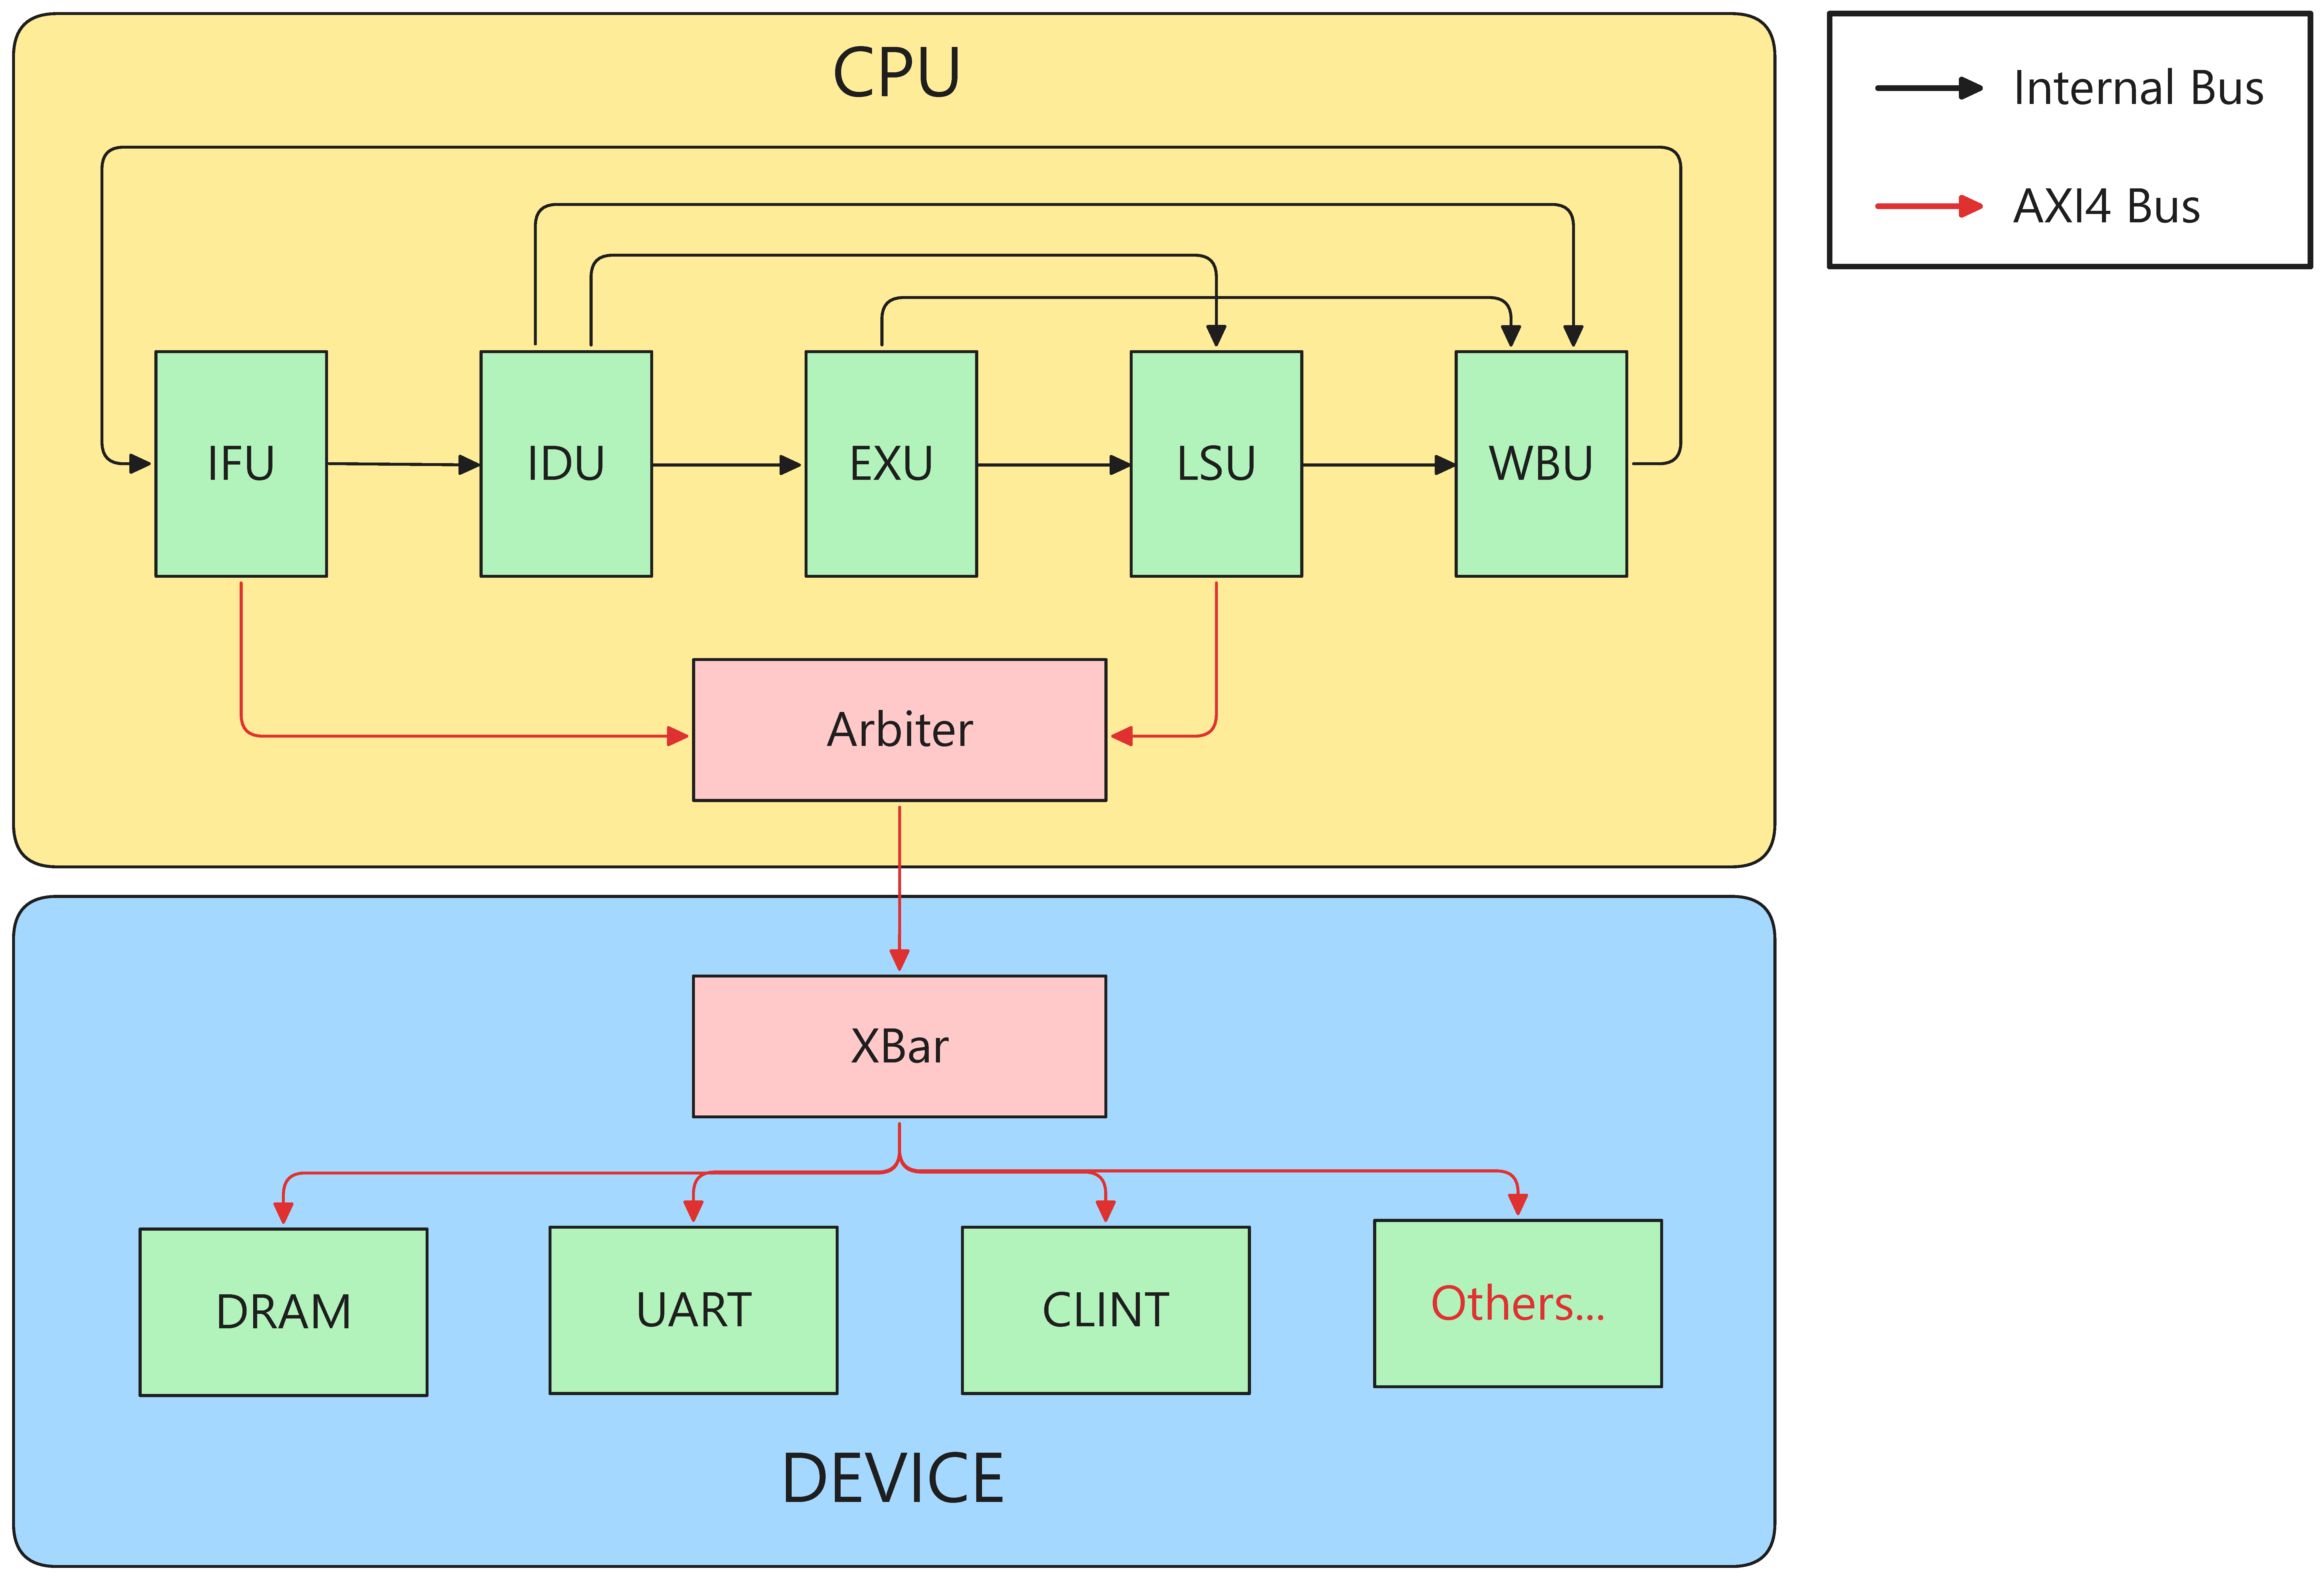
\includegraphics[width=0.8\textwidth]{image/bus.pdf}
	\caption{加入总线后的处理器结构图}
	\label{fig:bus}
\end{figure}

\section{系统优化}
目前,多周期处理器虽已能够支持基本程序的运行,但其性能表现仍存在明显局限。本节将深入探讨CPU的优化策略。在存储优化方面,将引入高速缓存技术,以显著提升数据访问效率,减少存储器访问延迟。在并行优化方面,将采用流水线技术,通过指令重叠执行增强处理器的并行处理能力,从而提高整体性能。这些优化措施旨在解决当前多周期处理器的性能瓶颈,为其在复杂计算任务中的应用奠定基础。

\subsection{存储优化——高速缓存}

针对存储器的层次结构,表\ref{tab:memorizer_level}展示了不同存储器的性能特点。可以看出,涉及访存的指令通常比其他指令耗时高几个量级。由于存储介质的物理限制,没有一种存储器能够同时满足大容量、高速度和低成本的要求。因此,计算机系统通常集成多种存储器,并通过特定技术将它们有机组织成层次结构,以在整体上实现大容量、高速度和低成本的综合性能。

\begin{table}[H]
	\centering
	\caption{存储器层次结构}
	\begin{tabularx}{\textwidth}{>{\centering\arraybackslash}X >{\centering\arraybackslash}X >{\centering\arraybackslash}X >{\centering\arraybackslash}X}
		\toprule
		\textbf{存储器} & \textbf{延迟} & \textbf{成本} & \textbf{容量} \\
		\midrule
		寄存器          & 约1ns        & 高           & 约1KB        \\
		主存(DRAM)     & 约10ns       & 中等          & 约10GB       \\
		外存(SSD)      & 约10us       & 低           & 约1TB        \\
		磁盘(HDD)      & 约10ms       & 低           & 约10TB       \\
		磁带           & 约10s        & 最低          & 大于10TB      \\
		\bottomrule
	\end{tabularx}
	\label{tab:memorizer_level}
\end{table}

为了理解存储层次结构的设计原因,需要引入程序局部性的概念:
\begin{enumerate}[label={\arabic*)}, itemsep=0pt, parsep=0pt]
	\item \textbf{时间局部性}:一旦访问某个存储单元,短时间内很可能会再次访问它,例如在循环结构中。
	\item \textbf{空间局部性}:一旦访问某个存储单元,短时间内很可能会访问其相邻单元,例如在数组遍历中。
\end{enumerate}


基于局部性原理,即使慢速存储器的容量很大,程序在一段时间内通常只会访问其中的一小部分数据。因此,可以将这部分数据从慢速存储器预取到快速存储器中,以便后续访问。这就是缓存(cache)的基本思想。为了优化访存效率,可以在寄存器和DRAM之间添加一层cache,在访问DRAM之前,先访问cache:如果所需数据已在cache中,则直接访问Cache中的数据;如果所需数据不在cache中,则先将数据从DRAM读入cache,然后再访问cache中的数据。

如图\ref{fig:cache_cpu}所示,在IFU和Arbiter之间引入指令缓存(icache),以加速指令的访问;在LSU和Arbiter之间引入数据缓存(dcache),以加速数据的读写操作。这种设计通过减少对主存的直接访问,显著降低访存延迟,从而提升处理器的整体性能。

\begin{figure}[htbp]
	\centering
	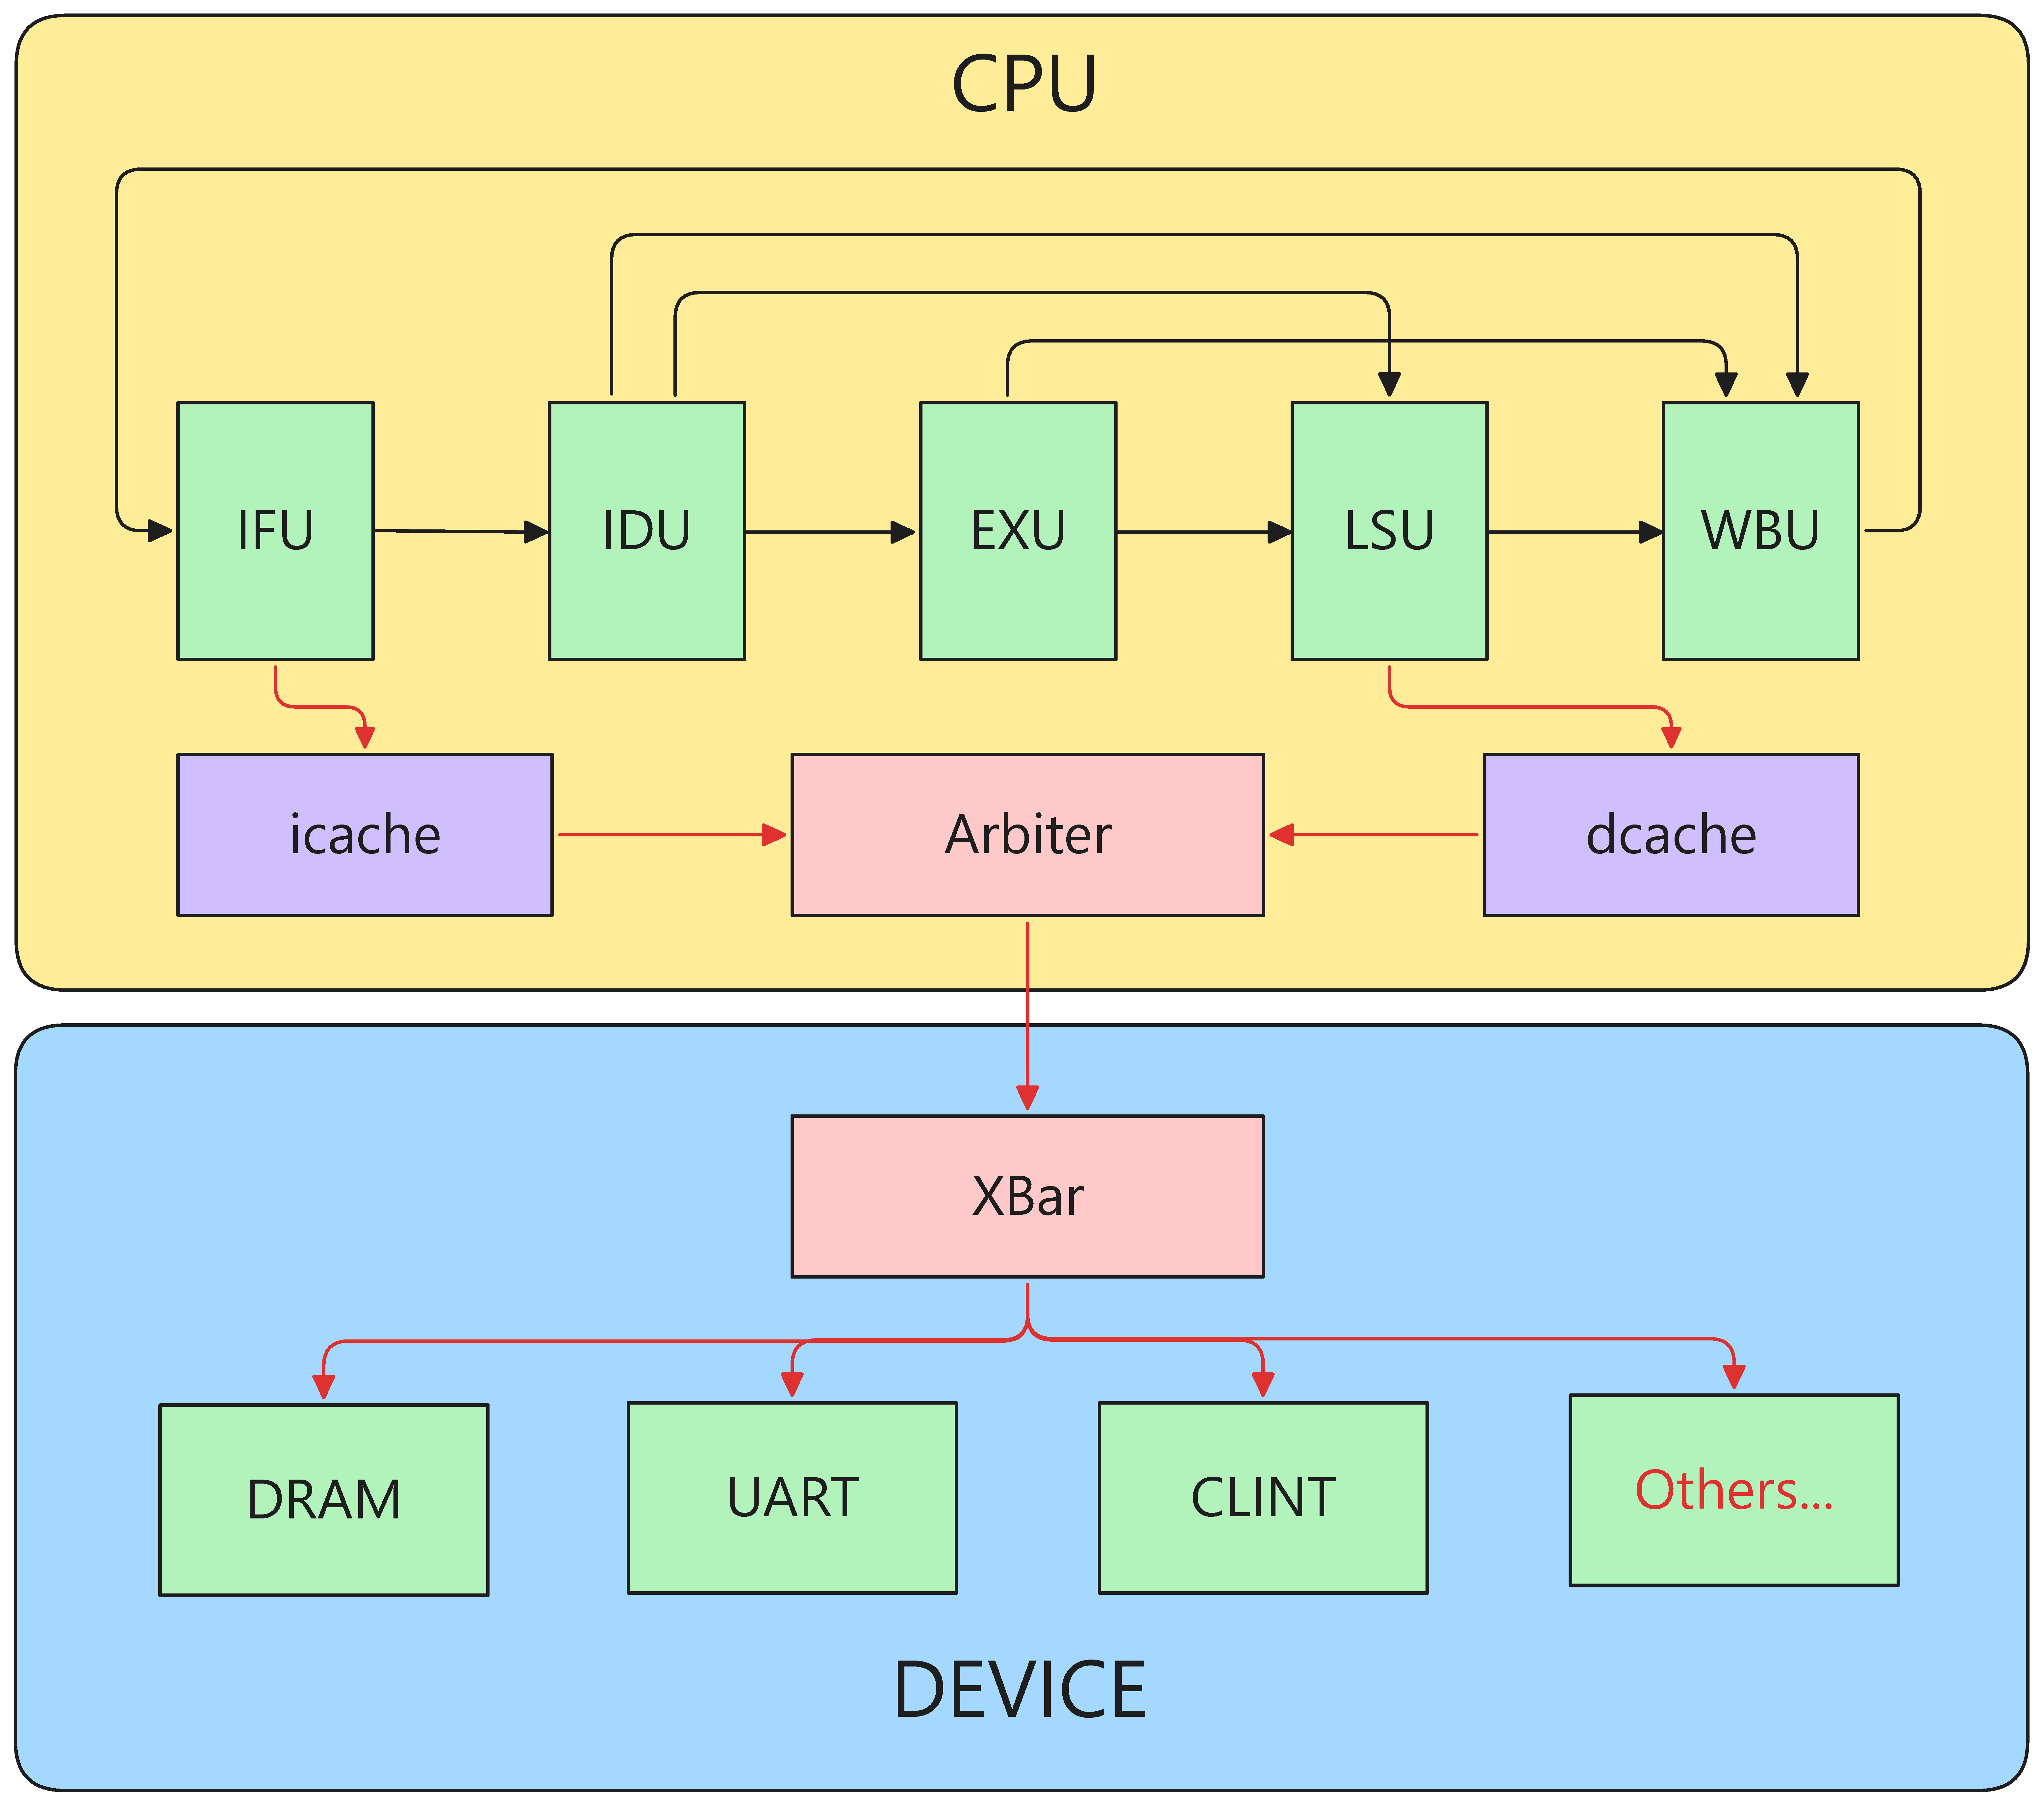
\includegraphics[width=0.6\textwidth]{image/cache_cpu.pdf}
	\caption{加入cache后的处理器结构图}
	\label{fig:cache_cpu}
\end{figure}

关于主存与缓存地址的映射方式,主要有以下三种,它们对缓存效率和性能的影响各不相同:
\begin{enumerate}[label={\arabic*)}, itemsep=0pt, parsep=0pt]
	\item \textbf{全相联映射}:全相联映射允许主存中的任意一个块映射到缓存中的任意一个位置。这种方式提供了最大的灵活性,因为主存中的每个块都可以放置在缓存的任何位置。然而,这种灵活性也带来了较高的查找成本,因为每次访问缓存时都需要检查所有缓存行,以确定是否存在所需的数据。优点是缓存利用率高,能够有效减少缓存缺失,但缺点是硬件实现复杂,查找速度较慢。
	\item \textbf{直接相联映射}:直接相联映射将主存中的每个块固定映射到缓存中的一个特定位置。具体来说,主存地址通过哈希函数(通常是取模操作)计算出缓存中的唯一位置。这种方式的查找速度非常快,因为每次访问缓存时只需要检查一个位置即可。优点是硬件实现简单,查找速度快,但缺点是缓存利用率较低,缓存缺失率较高。
	\item \textbf{组相联映射}:组相联映射是前两者的折中方案。它将缓存分为多个组,每个组包含多个缓存行。主存中的每个块可以映射到缓存中的一个特定组,但在组内可以自由选择缓存行。这种方式结合了直接相联映射的快速查找和全相联映射的高利用率,提供了较好的性能和硬件复杂度的平衡。组相联映射在查找速度和缓存利用率之间取得了较好的平衡,是现代缓存设计中最常用的方式。
\end{enumerate}

关于替换算法,由于程序运行一段时间后cache的空间会满,所以需要需要某种机制进行替换,主要的替换算法有以下四种:
\begin{enumerate}[label={\arabic*)}, itemsep=0pt, parsep=0pt]
	\item \textbf{随机替换(RR,Random Replacement)}:随机选择一个缓存行进行替换。这种方法简单易实现,但性能较差。
	\item \textbf{先进先出(FIFO,First-In-First-Out)}:替换最早进入缓存的行。这种方法基于时间顺序,简单且易于硬件实现,但可能导致频繁使用的数据被过早替换。
	\item \textbf{最不经常使用(LFU,Least Frequently Used)}:替换访问次数最少的缓存行。这种方法通过统计每个缓存行的访问频率来决定替换策略,适用于访问模式较为固定的场景。
	\item \textbf{近期最少使用(LRU,Least Recently Used)}:替换最近一段时间内最少使用的缓存行。这种方法基于时间局部性原理,能够较好地保留频繁访问的数据,是现代缓存设计中最常用的算法之一。
\end{enumerate}

\subsection{并行优化——流水线}
目前,处理器采用多周期设计,即执行一条指令需要多个时钟周期。为了提升指令执行的吞吐量,从而增强计算效率,流水线技术作为一种指令级并行方法被广泛应用。流水线通过将指令的执行过程分解为多个阶段,使得每个阶段可以在不同的时钟周期内并行处理,从而显著提高指令的吞吐量。如图\ref{fig:pipeline_timeline}所示,在处理器运行期间,各单元模块并行工作,极大地提升了整体吞吐量。

\begin{figure}[htbp]
	\centering
	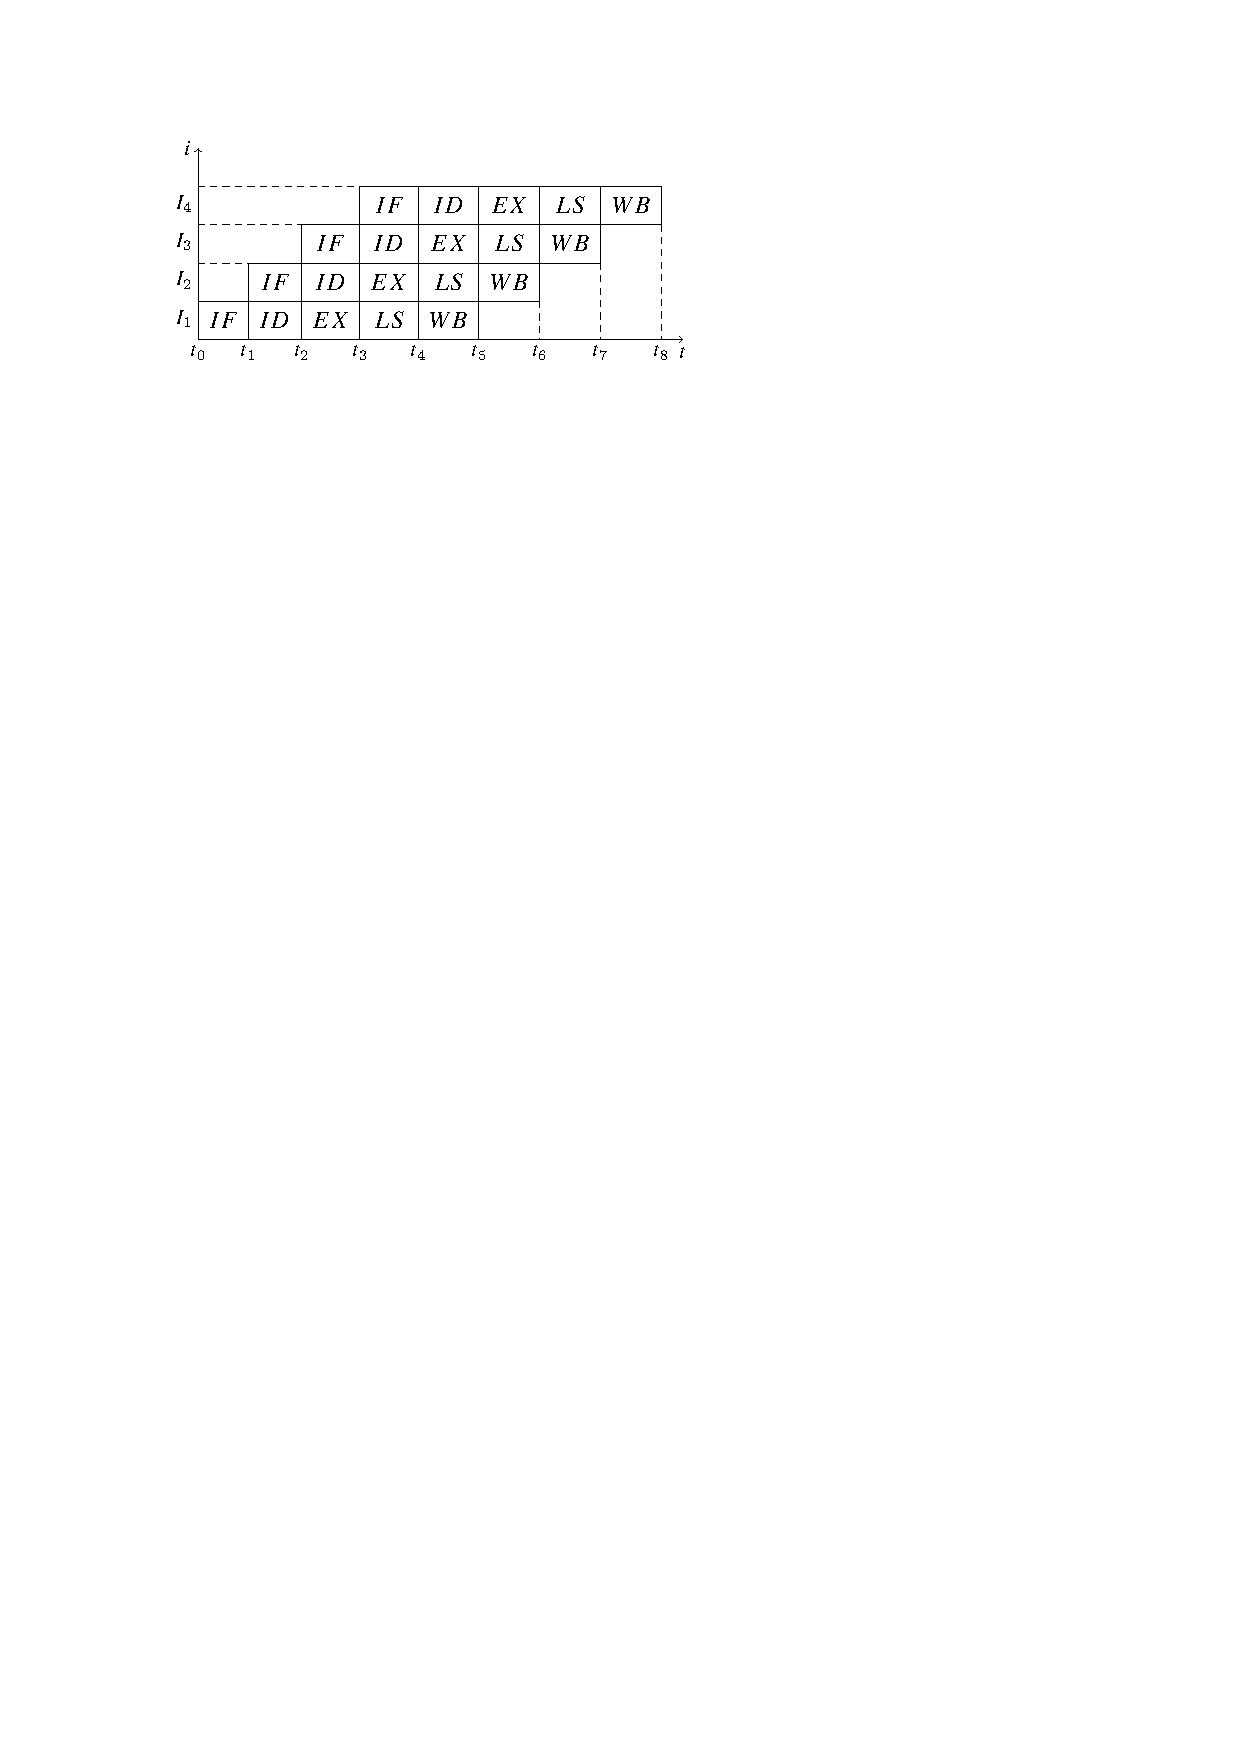
\includegraphics[width=0.8\textwidth]{image/pipeline_timeline.pdf}
	\caption{指令流水线时空图}
	\label{fig:pipeline_timeline}
\end{figure}

对于流水线处理器,可以通过让IFU持续取指,并在每个模块完成消息处理后立即向下游发送消息,从而实现高效并行处理。具体来说,只需在模块间添加流水线寄存器,并优化模块间通信逻辑,即可实现流水线设计。如图\ref{fig:assembly_line_cpu}所示,加入流水线技术后的处理器被划分为五个流水段,每个阶段负责特定的指令处理任务,从而实现高效的指令级并行。

\begin{figure}[htbp]
	\centering
	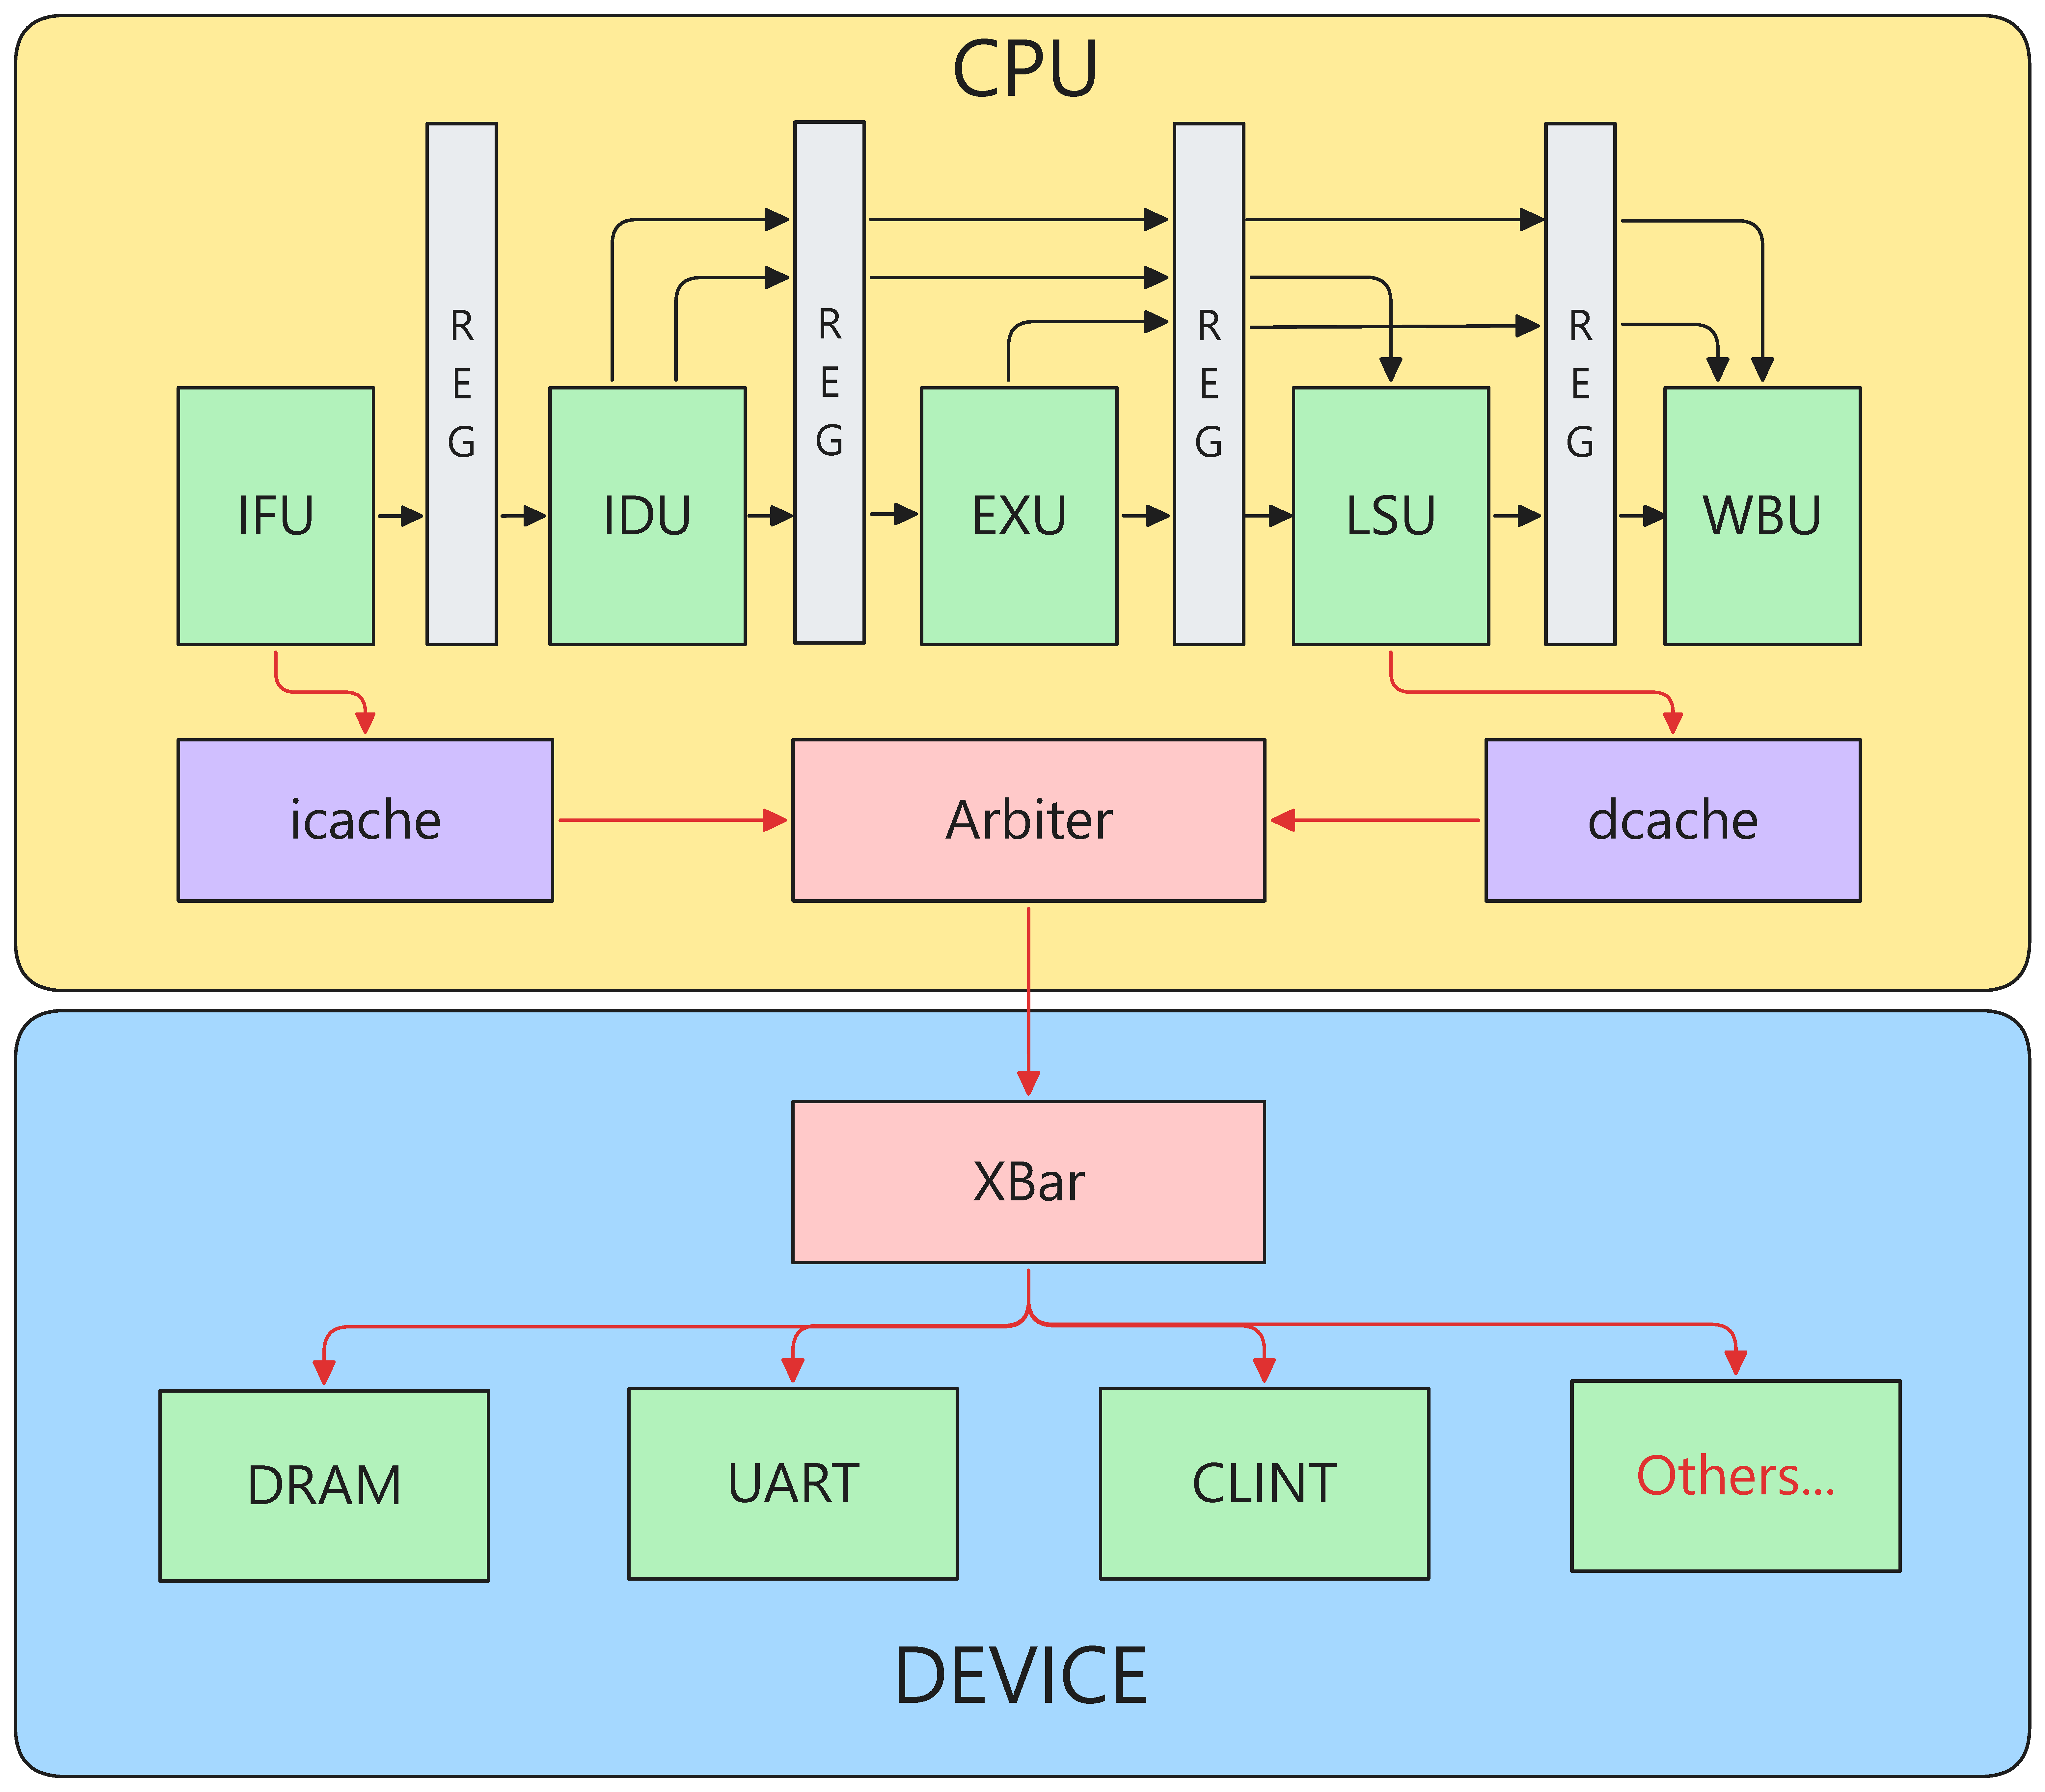
\includegraphics[width=0.6\textwidth]{image/assembly_line_cpu.pdf}
	\caption{加入流水线技术后的处理器结构图}
	\label{fig:assembly_line_cpu}
\end{figure}

流水线处理器中存在一些情况,可能导致当前指令无法按预期执行,这种情况称为冒险(Hazard)。若忽视冒险而强行执行指令,将导致CPU状态机的转移结果与ISA状态机不一致,表现为指令执行结果不符合其语义。因此,在流水线设计中,必须检测并解决冒险问题。冒险主要分为以下三类:

\begin{enumerate}[label={\arabic*)}, itemsep=0pt, parsep=0pt]
	\item \textbf{结构冒险}:由于硬件资源不足,导致多个指令同时竞争同一资源。例如,多个指令同时需要访问同一功能单元或总线。可以通过增加硬件资源的副本,以减少竞争;或通过调整指令执行顺序,避免资源冲突。
	\item \textbf{数据冒险}:由指令间的数据依赖关系引起。例如,后续指令需要使用前条指令尚未生成的结果。可以通过在流水线中插入空操作,确保数据准备好后再执行后续指令;或将后续指令所需的数据直接从上游阶段转发到下游阶段,避免等待。
	\item \textbf{控制冒险}:由分支指令引起,由于分支方向未确定,处理器无法立即确定后续指令的取指地址。可以通过使用硬件预测器猜测分支方向,提前取指后续指令;或将分支指令后的几条指令延迟执行,确保分支方向确定后再继续。
\end{enumerate}

\section{本章小结}
本章针对处理器在访问存储器和外围设备时存在的延迟问题,引入了总线协议,并采用缓存技术和流水线技术分别优化访存效率和提升并行处理能力。通过这些改进,已完成一款五级流水线的 RISC-V 处理器设计方案。与单周期处理器相比,该方案不仅显著提升了处理器性能,还使其能够在真实环境中实现流片生产,为实际应用奠定了坚实基础。